\documentclass[11pt,a4paper]{article}
\usepackage[T1]{fontenc}
\usepackage[utf8]{inputenc}
\usepackage[margin=1in]{geometry}
\usepackage{amsmath,amssymb}
\usepackage{longtable}
\usepackage{booktabs}
\usepackage{array}
\usepackage{enumitem}
\usepackage{tikz}
\usepackage{hyperref}
\hypersetup{colorlinks=true, linkcolor=black!40!black, citecolor=black, urlcolor=black,
            pdftitle={The Top-Down Cascade Method for Stacked Friction Systems}}

\setlength{\parindent}{0pt}
\setlength{\parskip}{6pt}

\title{\textbf{The Top-Down Cascade Method for Stick--Slip Analysis\\ in Stacked Friction Systems}\\[4pt]
\large (the SLIP-SPLIT-CALCULATE Algorithm)}
\date{\today}

\begin{document}
\maketitle

\begin{abstract}
This paper presents a hand-calculation procedure, the Top-Down Cascade Method, for finding the instantaneous acceleration of every block in a vertical stack of rigid bodies coupled by dry friction, where each block may carry an independent horizontal driving force and the coefficients of static and kinetic friction are equal at every interface. Rather than solving the equations of motion for the whole stack at once against an assumed pattern of sticking and slipping interfaces, the method proceeds sequentially from the top of the stack downward. It tests a running drive force against each interface in turn, merges blocks that stick into a temporary rigid group, and transmits the limiting friction of any interface that slips to the block beneath it. A fail-safe check, the internal shear verification, is applied to every group formed by sticking, so that a group is never left in a state that its own internal friction could not actually sustain. The method is demonstrated in full on a thirty-block system in which several groups form and subsequently fracture at more than one point along the stack, producing a complete, self-consistent set of accelerations using only arithmetic that can be carried out by hand.
\end{abstract}

\tableofcontents

\section{Introduction}

Stacks of rigid blocks coupled through dry friction appear throughout mechanics: crates stacked on a loading pallet, plates in a friction clutch, sedimentary layers under lateral load, and idealized models of granular columns are all systems in which a horizontal force applied to one member may or may not reach its neighbours, depending on whether the friction between them can sustain the shear force involved.

For a stack of $n$ blocks there are, in general, $n$ frictional interfaces, including the base if the stack rests on a fixed floor, and each interface is either sticking or slipping. A fully rigorous treatment would propose a pattern of sticking and slipping across all $n$ interfaces, solve the resulting equations of motion for that pattern, and then check that the friction force implied at every sticking interface stays within its static limit and that the sliding direction assumed at every slipping interface is consistent with the result. Because the number of candidate patterns grows quickly with $n$, and because a change at one interface can alter the required force at every other interface in its group, this approach becomes impractical to carry out by hand once $n$ passes four or five blocks.

This paper presents an alternative, the Top-Down Cascade Method, that resolves the whole configuration through a single descending pass with local checks, without solving for the entire stack at once or guessing a global stick--slip pattern in advance. Because the coefficients of static and kinetic friction are taken as equal at every interface, the largest force an interface can sustain while sticking is also the exact force it exerts while slipping. This single fact is what allows the friction released by a slipping interface to be carried downward and treated as a known, fixed load on the next block, rather than as a further unknown.

The method is a heuristic rather than a general proof of correctness: it relies on the direction of sliding at each interface being given, unambiguously, by the sign of the net drive force computed at the moment that interface is tested. This condition held throughout the thirty-block case examined in Section~\ref{sec:application}, and the method is best regarded as a practical calculation tool for problems of this class rather than as a substitute for a full numerical treatment of pathological or near-degenerate loadings.

\section{Problem Definition and Notation}
\label{sec:problem}

Consider $n$ rigid blocks arranged in a vertical column and labelled $1$ (top) to $n$ (bottom); block $n$ rests on a fixed floor. Block $i$ has mass $m_i$ and may carry an external horizontal force $F_i$, applied directly to that block and independent of the force on any other block. A single global horizontal axis is fixed for the entire problem, with rightward taken as positive; every force, velocity, and acceleration in this paper is a signed scalar measured along that axis.

Blocks $i$ and $i+1$ meet at a horizontal interface, denoted interface $i$, for $i = 1, \dots, n-1$; interface $n$ is the contact between block $n$ and the fixed floor. Each interface has a limiting friction force $f_i > 0$, set by the normal force transmitted across it (the combined weight of every block above it) and the coefficient of friction there. Because $\mu_s = \mu_k$ at every interface, $f_i$ serves two purposes at once: it is the largest shear force the interface can sustain without slipping, and it is also the magnitude of the kinetic friction it exerts once it does slip. Table~\ref{tab:input} lists $m_i$, $F_i$, and $f_i$ for the thirty-block system examined in Section~\ref{sec:application}.

Figure~\ref{fig:schematic} shows three consecutive blocks from the interior of such a stack, indicating the sign convention and the friction exchanged at each interface.

\begin{figure}[h]
\centering
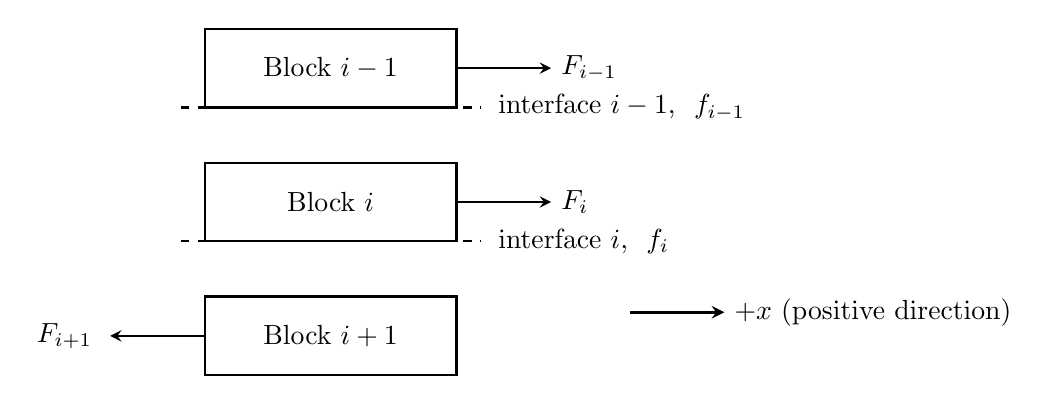
\begin{tikzpicture}[>=stealth, thick, scale=1]
 \draw (0,6) rectangle (3.2,7);
 \node at (1.6,6.5) {Block $i-1$};
 \draw[->] (3.2,6.5) -- (4.4,6.5);
 \node[right] at (4.4,6.5) {$F_{i-1}$};
 \draw[dashed] (-0.3,6) -- (3.5,6);
 \node[right] at (3.6,6) {interface $i-1$, \ $f_{i-1}$};

 \draw (0,4.3) rectangle (3.2,5.3);
 \node at (1.6,4.8) {Block $i$};
 \draw[->] (3.2,4.8) -- (4.4,4.8);
 \node[right] at (4.4,4.8) {$F_i$};
 \draw[dashed] (-0.3,4.3) -- (3.5,4.3);
 \node[right] at (3.6,4.3) {interface $i$, \ $f_i$};

 \draw (0,2.6) rectangle (3.2,3.6);
 \node at (1.6,3.1) {Block $i+1$};
 \draw[<-] (-1.2,3.1) -- (0,3.1);
 \node[left] at (-1.3,3.1) {$F_{i+1}$};

 \draw[->, line width=1pt] (5.4,3.4) -- (6.6,3.4);
 \node[right] at (6.6,3.4) {$+x$ (positive direction)};
\end{tikzpicture}
\caption{General arrangement of three consecutive blocks. Each block carries its own external force, applied along the single global axis; each interface below a block has a limiting friction force $f_i$, equal in magnitude whether that interface is sticking or slipping.}
\label{fig:schematic}
\end{figure}

\section{The Top-Down Cascade Method}
\label{sec:method}

The method proceeds in four phases. Phase~I is carried out once, at the outset. Phase~II is repeated as each new block is reached while scanning down the stack. Phase~III is the rule by which a result already found for one block or group is passed to the block beneath it. Phase~IV is a fail-safe check applied whenever blocks have been provisionally grouped by sticking, and it is what allows such a group to be broken apart correctly, layer by layer, when it cannot in fact remain rigid.

\subsection{Phase 1: System Initialization}

Fix the global sign convention once, before any block is examined, and compute the limiting friction $f_i$ at every interface from the normal force transmitted across it. All forces used afterward are signed quantities measured along this single axis, and this axis is not changed for the remainder of the calculation.

\subsection{Phase 2: Boundary Evaluation (Top-Down Progression)}

Working down from the top of the stack, maintain a candidate group that begins as a single block and may grow as further blocks are added to it. Suppose the group currently spans blocks $p$ through $q$ (initially $p = q = 1$), and let $C$ denote the force transmitted into this group from whatever lies immediately above block $p$ ($C = 0$ if $p = 1$). The drive on the group is
\begin{equation}
D \;=\; C + \sum_{i=p}^{q} F_i .
\label{eq:drive}
\end{equation}
Compare $|D|$ with $f_q$, the limiting friction of the interface directly beneath the group.
\begin{itemize}[leftmargin=1.4em]
\item If $|D| \le f_q$: interface $q$ holds. Block $q+1$ is added to the group ($q \to q+1$), and the comparison in Equation~\eqref{eq:drive} is repeated against the new value of $f_q$.
\item If $|D| > f_q$: interface $q$ yields. If the group is a single block ($p=q$), its acceleration is found immediately (Equation~\eqref{eq:stateA} below). If the group contains more than one block, its members cannot be assigned this acceleration until it has been checked that every interface between them can actually sustain it; that check is Phase~IV.
\end{itemize}

\subsection{Phase 3: Load Transmission (The Cascade)}

Once a block or group's acceleration has been finalized, the interface immediately beneath it is, by construction, the one that was found to yield. That interface exerts a kinetic friction force of magnitude equal to its own limiting value, directed the same way the group above it is sliding, onto the block immediately below. This transmitted force becomes the new carried-in force $C$ for the next, still-unresolved part of the stack, and Phase~II resumes there.

For a single block that yields on its own (a group of size one), the acceleration follows directly:
\begin{equation}
a \;=\; \frac{D - f\,\mathrm{sgn}(D)}{m},
\label{eq:stateA}
\end{equation}
where $m$ is the block's mass, $f$ is the limiting friction of the interface directly beneath it, and $\mathrm{sgn}(D) = +1$ if $D>0$ and $-1$ if $D<0$. The quantity $f\,\mathrm{sgn}(D)$ is the value carried forward to the next block under this phase.

\subsection{Phase 4: Internal Shear Verification (The Fail-Safe)}

Suppose Phase~II has extended a candidate group across blocks $p$ through $q$ before finding that interface $q$ yields under drive $D$. Because the group has more than one member, its acceleration cannot be accepted until every interface between blocks $p$ and $q$ has been shown able to carry the force that a shared acceleration would require of it.

First, the acceleration the whole group would have if it stayed rigid while sliding at interface $q$ is
\begin{equation}
a^{(0)} \;=\; \frac{D - f_q\,\mathrm{sgn}(D)}{\displaystyle\sum_{i=p}^{q} m_i}.
\label{eq:a0}
\end{equation}
Then, starting at the interface immediately above the one that yielded (interface $q-1$) and working upward, each internal interface $j$ ($j = q-1, q-2, \dots, p$) is checked in turn. The force interface $j$ would need to supply, if blocks $p$ through $j$ are to share the acceleration $a^{(0)}$, is
\begin{equation}
F_{\mathrm{req}}(j) \;=\; \Big(\sum_{i=p}^{j} m_i\Big) a^{(0)} \;-\; \Big(C + \sum_{i=p}^{j} F_i\Big).
\label{eq:freq}
\end{equation}
If $|F_{\mathrm{req}}(j)| \le f_j$, interface $j$ holds under this assumption, and the check continues at $j-1$. The first interface $j^{*}$ found, moving upward from $q-1$, at which $|F_{\mathrm{req}}(j)|$ exceeds $f_j$ is where the group actually fractures: blocks $p$ through $j^{*}$ remain a smaller candidate group, still carrying the original input $C$, while blocks $j^{*}+1$ through $q$ separate and are driven from above by the friction of the interface that has just failed, $f_{j^{*}}\,\mathrm{sgn}(a^{(0)})$. If the separated portion is a single block, its acceleration follows directly from Equation~\eqref{eq:stateA}; if it still contains more than one block, it is itself resubmitted to Phase~IV, with $a^{(0)}$ recomputed for the smaller group. If no interface fails during the scan, the entire group $p$ through $q$ moves together at $a^{(0)}$, and this is its final acceleration.

Because a fracture always shortens the group under consideration, and Phase~IV is reapplied to each fragment it produces, the process terminates after at most $q-p$ fractures, each one resolved by Equations~\eqref{eq:a0} and \eqref{eq:freq}.

\subsection{Summary of the Procedure}

\begin{enumerate}[leftmargin=1.6em]
\item Fix the sign convention and compute $f_i$ for every interface (Phase~I).
\item Starting at block $1$ with $C=0$, extend a candidate group one block at a time, accumulating the drive $D$ of Equation~\eqref{eq:drive}, until the interface beneath the group yields (Phase~II).
\item If the group is a single block, find its acceleration directly from Equation~\eqref{eq:stateA} and go to step 5.
\item If the group has more than one block, compute $a^{(0)}$ from Equation~\eqref{eq:a0} and scan the internal interfaces upward from the one that just yielded, using Equation~\eqref{eq:freq}; split at the first interface that cannot supply the required force, and resolve each fragment, repeating this step for any fragment that still has more than one block (Phase~IV).
\item Transmit the limiting friction of the interface directly below the block or fragment just finalized to the next block down, as the new carried-in force $C$, and return to step 2 for the remainder of the stack (Phase~III).
\item Stop once every block has been assigned an acceleration.
\end{enumerate}

\section{Application to a Thirty-Block System}
\label{sec:application}

\subsection{System Data}

Table~\ref{tab:input} lists the mass, external force, and interface limiting friction for each of the thirty blocks used to test the method. Blocks are numbered from the top of the stack (block~1) to the bottom (block~30, in contact with the fixed floor through interface~30).

\begin{longtable}{c c c c}
\caption{Input data for the thirty-block system.}\label{tab:input}\\
\toprule
Block & Mass (kg) & External force (N) & $f_i$ (N) \\
\midrule
\endfirsthead
\toprule
Block & Mass (kg) & External force (N) & $f_i$ (N) \\
\midrule
\endhead
\midrule
\endfoot
\bottomrule
\endlastfoot
1  & 12 & $+3000$ & 58.8 \\
2  & 3  & $0$     & 61.5 \\
3  & 2  & $0$     & 100.3 \\
4  & 13 & $0$     & 105.0 \\
5  & 6  & $0$     & 151.2 \\
6  & 5  & $-2000$ & 217.3 \\
7  & 5  & $0$     & 207.0 \\
8  & 4  & $+1500$ & 270.0 \\
9  & 13 & $-2000$ & 270.9 \\
10 & 3  & $0$     & 316.8 \\
11 & 12 & $+2000$ & 171.6 \\
12 & 13 & $0$     & 263.9 \\
13 & 10 & $0$     & 323.2 \\
14 & 3  & $-1500$ & 239.2 \\
15 & 11 & $+2500$ & 333.5 \\
16 & 8  & $0$     & 295.2 \\
17 & 2  & $0$     & 387.5 \\
18 & 2  & $0$     & 571.5 \\
19 & 3  & $-2000$ & 455.0 \\
20 & 5  & $0$     & 472.5 \\
21 & 5  & $0$     & 392.0 \\
22 & 10 & $0$     & 465.0 \\
23 & 11 & $+2500$ & 917.7 \\
24 & 2  & $0$     & 749.8 \\
25 & 10 & $0$     & 761.2 \\
26 & 5  & $-2500$ & 480.6 \\
27 & 13 & $0$     & 935.9 \\
28 & 12 & $0$     & 548.1 \\
29 & 13 & $0$     & 756.0 \\
30 & 10 & $+2500$ & 1356.0 \\
\end{longtable}

\subsection{Outcome}

Applying the procedure of Section~\ref{sec:method} block by block, exactly as carried out in Appendix~\ref{app:derivation}, gives the final acceleration of every block, listed in Table~\ref{tab:results}. Where two or more blocks share a row, the internal shear check of Phase~IV confirmed that they remain stuck together and move with a common acceleration; all other blocks are independent, having separated from their neighbours through one or more fractures.

\begin{longtable}{c c l}
\caption{Final accelerations for the thirty-block system.}\label{tab:results}\\
\toprule
Block(s) & Acceleration (m/s$^2$) & State \\
\midrule
\endfirsthead
\toprule
Block(s) & Acceleration (m/s$^2$) & State \\
\midrule
\endhead
\midrule
\endfoot
\bottomrule
\endlastfoot
1        & $+245.10$ & independent \\
2        & $-0.90$   & independent \\
3, 4     & $-2.90$   & move together \\
5        & $-7.70$   & independent \\
6        & $-326.30$ & independent \\
7        & $-2.06$   & independent \\
8        & $+255.75$ & independent \\
9        & $-112.24$ & independent \\
10       & $+15.30$  & independent \\
11       & $+125.97$ & independent \\
12, 13   & $-6.59$   & move together \\
14       & $-312.53$ & independent \\
15       & $+175.21$ & independent \\
16       & $+4.79$   & independent \\
17       & $-46.15$  & independent \\
18       & $-92.00$  & independent \\
19       & $-324.50$ & independent \\
20, 21   & $-6.30$   & move together \\
22       & $+7.30$   & independent \\
23       & $+101.57$ & independent \\
24       & $+83.95$  & independent \\
25       & $-1.14$   & independent \\
26       & $-251.64$ & independent \\
27, 28   & $+2.70$   & move together \\
29       & $+15.99$  & independent \\
30       & $+38.80$  & independent \\
\end{longtable}

\subsection{Observations}

Eight temporary stuck groups form during the top-down pass, ranging in initial size from two to five blocks. One of them, blocks 20 and 21, passes its internal check on the first attempt and stays paired through to the final result. Three more groups -- opening at block 2, at block 12, and at block 27 -- lose one or more members to internal fracture but still end with a residual pair moving together (blocks 3 and 4; blocks 12 and 13; blocks 27 and 28, respectively). The remaining four groups -- spanning blocks 10--11, 17--19, 22--23, and 25--26 -- fracture all the way down to individual blocks, with none of their original members staying paired. In total, the calculation involves eleven internal-fracture events, three of which occur in succession within the very first group examined, blocks 2 through 6.

Seven blocks -- 1, 7, 8, 9, 15, 16, and 24 -- slip on their very first check, without ever forming a group: the drive reaching each of them already exceeds the friction of the interface immediately below.

The resulting accelerations span a wide range, from about $0.9\ \text{m/s}^2$ in magnitude (block 2) to over $300\ \text{m/s}^2$ (block 6). This spread reflects the particular combination of small block masses and large transmitted or applied forces chosen for this test case, and is not a general property of the method itself.

\section{Discussion}

The chief practical advantage of the Top-Down Cascade Method is that it never requires solving for more than one small group of blocks at a time, and each such calculation is a short linear equation together with a handful of inequality checks. A direct approach that tried to solve the whole thirty-block stack as one system, without first knowing which interfaces slip, would need to work through an unmanageable number of candidate stick--slip patterns; the method presented here instead discovers the correct pattern layer by layer, using only the sign of a running drive force and a single provisional-acceleration check at each stuck group.

The method's reliability rests on one assumption worth stating plainly: at every interface that yields, the direction of sliding is taken to be the sign of the net drive force computed at the moment that interface is tested. This is the natural assumption to make, and it held at every interface in the case examined here, but it is an assumption rather than something proved from first principles at each step. A configuration in which the correct sliding direction at some interface is not simply the sign of the locally computed drive would call for closer inspection than the method provides on its own. Within that scope, the method gives a complete, self-consistent set of accelerations for a stack of any size using only arithmetic that can be carried out by hand, in the time frame of an examination or a written problem set rather than that of a numerical solver.

\section{Conclusion}

The Top-Down Cascade Method reduces the problem of finding the acceleration of every block in a frictionally coupled stack to a short sequence of local decisions: test a running drive force against the interface below it, merge blocks that stick, and verify, rather than assume, that any group formed this way can actually remain rigid before accepting its acceleration as final. Applied to a thirty-block system with eight temporary groups and eleven internal fractures, the method produced a complete set of accelerations using only the arithmetic set out in Section~\ref{sec:application} and Appendix~\ref{app:derivation}, without recourse to matrix methods or iterative solvers.

\appendix
\section{Full Derivation for the Thirty-Block System}
\label{app:derivation}

This appendix carries out the method of Section~\ref{sec:method} in full for every block of the system defined in Table~\ref{tab:input}, grouped by cascade in the order in which the top-down pass reaches them.

\subsection{Blocks 1--6}

\paragraph{Block 1 ($m=12$ kg).} The drive on block 1 is its external force alone, $D=+3000$ N. Since $|3000| > f_1 = 58.8$ N, interface 1 yields, giving
\[
a_1 = \frac{3000 - 58.8}{12} = 245.10\ \text{m/s}^2 .
\]
Block 1 transmits $+58.8$ N to block 2.

\paragraph{Blocks 2--5 (group forming).} Block 2 ($D=+58.8$ N) has $f_2 = 61.5$ N, which holds, so block 2 merges with block 3. Block 3 ($D=+58.8$ N) has $f_3 = 100.3$ N, which holds, merging with block 4. Block 4 ($D=+58.8$ N) has $f_4 = 105.0$ N, which holds, merging with block 5. Block 5 ($D=+58.8$ N) has $f_5 = 151.2$ N, which also holds, merging with block 6, which carries an external force of $-2000$ N.

\paragraph{Group (2--6) boundary check.} The drive on the group is $D = 58.8 - 2000 = -1941.2$ N. Since $f_6 = 217.3$ N and $|{-1941.2}| > 217.3$, interface 6 yields.

\paragraph{Internal shear verification, group (2--6), total mass 29 kg.}
\[
a^{(0)} = \frac{-1941.2 + 217.3}{29} = -59.44\ \text{m/s}^2 .
\]
Checking interface 5 (blocks 2--5 against block 6), with mass of (2--5) equal to 24 kg:
\[
F_{\mathrm{req}} = 24(-59.44) = -1426.6\ \text{N}, \qquad \text{required at interface 5} = -1426.6 - 58.8 = -1485.4\ \text{N}.
\]
Since $f_5 = 151.2$ N is far smaller than $1485.4$ N, interface 5 fails: the group fractures there, and block 6 separates.

\paragraph{Block 6 (isolated).} Driven by its external $-2000$ N, dragged by $-151.2$ N from interface 5 above (block 5 now slipping against it), and resisted by $+217.3$ N from interface 6 below:
\[
a_6 = \frac{-2000+151.2+217.3}{5} = \frac{-1631.5}{5} = -326.30\ \text{m/s}^2 .
\]

\paragraph{Group (2--5), recomputed.} Now driven by $+58.8$ N from above and $-151.2$ N from below:
\[
D = 58.8 - 151.2 = -92.4\ \text{N}, \qquad a^{(0)} = \frac{-92.4}{24} = -3.85\ \text{m/s}^2 .
\]
Checking interface 4 (blocks 2--4 against block 5), with mass of (2--4) equal to 18 kg:
\[
F_{\mathrm{req}} = 18(-3.85) = -69.3\ \text{N}, \qquad \text{required at interface 4} = -69.3 - 58.8 = -128.1\ \text{N}.
\]
Since $f_4 = 105.0$ N $< 128.1$ N, interface 4 fails: block 5 separates.

\paragraph{Block 5 (isolated).} Driven by $-151.2$ N from below and $+105.0$ N from interface 4 above:
\[
a_5 = \frac{-151.2+105.0}{6} = -7.70\ \text{m/s}^2 .
\]

\paragraph{Group (2--4), recomputed.} Now driven by $+58.8$ N from above and $-105.0$ N from below:
\[
D = 58.8 - 105.0 = -46.2\ \text{N}, \qquad a^{(0)} = \frac{-46.2}{18} = -2.56\ \text{m/s}^2 .
\]
Interface 3 (blocks 2--3 against block 4) is checked in the same way and is found to hold; the next candidate boundary, interface 2, is checked below.

\paragraph{Checking interface 2 (block 2 against blocks 3--4).} With mass of block 2 alone equal to 3 kg:
\[
F_{\mathrm{req}} = 3(-2.56) = -7.68\ \text{N}, \qquad \text{required at interface 2} = -7.68 - 58.8 = -66.48\ \text{N}.
\]
Since $f_2 = 61.5$ N $< 66.48$ N, interface 2 fails: block 2 separates.

\paragraph{Block 2 (isolated).} Driven by $+58.8$ N from above and $-61.5$ N from interface 2 below:
\[
a_2 = \frac{58.8-61.5}{3} = -0.90\ \text{m/s}^2 .
\]

\paragraph{Blocks 3--4 (remaining pair).} Now driven by $+61.5$ N (the friction just released at interface 2) from above and $-105.0$ N from below:
\[
D = 61.5-105.0 = -43.5\ \text{N}, \qquad a_{3,4} = \frac{-43.5}{15} = -2.90\ \text{m/s}^2 .
\]
Interface 3 continues to hold at this final acceleration, so blocks 3 and 4 move together.

Block 6 transmits $-217.3$ N to block 7.

\subsection{Blocks 7--11}

\paragraph{Block 7 ($m=5$ kg).} $D=-217.3$ N; $f_7 = 207.0$ N; $|{-217.3}|>207.0$, yields.
\[
a_7 = \frac{-217.3+207.0}{5} = -2.06\ \text{m/s}^2 .
\]
Transmits $-207.0$ N to block 8.

\paragraph{Block 8 ($m=4$ kg, external $+1500$ N).} $D = 1500-207.0 = 1293.0$ N; $f_8 = 270.0$ N; yields.
\[
a_8 = \frac{1293.0-270.0}{4} = 255.75\ \text{m/s}^2 .
\]
Transmits $+270.0$ N to block 9.

\paragraph{Block 9 ($m=13$ kg, external $-2000$ N).} $D = -2000+270.0 = -1730.0$ N; $f_9 = 270.9$ N; yields.
\[
a_9 = \frac{-1730.0+270.9}{13} = -112.24\ \text{m/s}^2 .
\]
Transmits $-270.9$ N to block 10.

\paragraph{Blocks 10--11.} Block 10 ($D=-270.9$ N) has $f_{10}=316.8$ N, which holds, merging with block 11, which carries an external force of $+2000$ N.

\paragraph{Group (10,11) boundary check.} $D = -270.9+2000 = 1729.1$ N; $f_{11}=171.6$ N; yields.

\paragraph{Internal shear verification, mass 15 kg.}
\[
a^{(0)} = \frac{1729.1-171.6}{15} = 103.83\ \text{m/s}^2 .
\]
Checking interface 10 (the only internal interface in this pair), with mass of block 10 alone equal to 3 kg:
\[
F_{\mathrm{req}} = 3(103.83) = 311.5\ \text{N}, \qquad \text{required at interface 10} = 311.5-(-270.9) = 582.4\ \text{N}.
\]
Since $f_{10}=316.8$ N $< 582.4$ N, interface 10 fails: the pair separates completely.

\paragraph{Block 10 (isolated).} Driven by $-270.9$ N from above and $+316.8$ N from interface 10 below:
\[
a_{10} = \frac{-270.9+316.8}{3} = 15.30\ \text{m/s}^2 .
\]

\paragraph{Block 11 (isolated).} Driven by its external $+2000$ N and $-316.8$ N from interface 10 above, giving $2000-316.8=1683.2$ N, then resisted by $-171.6$ N from interface 11 below:
\[
a_{11} = \frac{1683.2-171.6}{12} = 125.97\ \text{m/s}^2 .
\]

Block 11 transmits $+171.6$ N to block 12.

\subsection{Blocks 12--14}

\paragraph{Blocks 12--13.} Block 12 ($m=13$ kg, $D=+171.6$ N) has $f_{12}=263.9$ N, which holds, merging with block 13. Block 13 ($m=10$ kg, $D=+171.6$ N) has $f_{13}=323.2$ N, which also holds, merging with block 14, which carries an external force of $-1500$ N.

\paragraph{Group (12--14) boundary check.} $D = 171.6-1500 = -1328.4$ N; $f_{14}=239.2$ N; yields.

\paragraph{Internal shear verification, mass 26 kg.}
\[
a^{(0)} = \frac{-1328.4+239.2}{26} = -41.88\ \text{m/s}^2 .
\]
Checking interface 13 (blocks 12--13 against block 14), with mass of (12,13) equal to 23 kg:
\[
F_{\mathrm{req}} = 23(-41.88) = -963.2\ \text{N}, \qquad \text{required at interface 13} = -963.2-171.6 = -1134.8\ \text{N}.
\]
Since $f_{13}=323.2$ N is far smaller, interface 13 fails: block 14 separates.

\paragraph{Block 14 (isolated).} Driven by its external $-1500$ N, dragged by $+323.2$ N from interface 13 above, and resisted by $+239.2$ N from interface 14 below:
\[
a_{14} = \frac{-1500+323.2+239.2}{3} = \frac{-937.6}{3} = -312.53\ \text{m/s}^2 .
\]

\paragraph{Group (12,13), recomputed.} Now driven by $+171.6$ N from above and $-323.2$ N from below:
\[
D = 171.6-323.2 = -151.6\ \text{N}, \qquad a^{(0)} = \frac{-151.6}{23} = -6.59\ \text{m/s}^2 .
\]
Checking interface 12 (block 12 against block 13), with mass of block 12 alone equal to 13 kg:
\[
F_{\mathrm{req}} = 13(-6.59) = -85.67\ \text{N}, \qquad \text{required at interface 12} = -85.67-171.6 = -257.27\ \text{N}.
\]
Since $f_{12}=263.9$ N $> 257.27$ N, interface 12 holds: blocks 12 and 13 move together at $-6.59$ m/s$^2$.

Block 14 transmits $-239.2$ N to block 15.

\subsection{Blocks 15--19}

\paragraph{Block 15 ($m=11$ kg, external $+2500$ N).} $D = 2500-239.2 = 2260.8$ N; $f_{15}=333.5$ N; yields.
\[
a_{15} = \frac{2260.8-333.5}{11} = 175.21\ \text{m/s}^2 .
\]
Transmits $+333.5$ N to block 16.

\paragraph{Block 16 ($m=8$ kg, no external force).} $D=+333.5$ N; $f_{16}=295.2$ N; yields.
\[
a_{16} = \frac{333.5-295.2}{8} = 4.79\ \text{m/s}^2 .
\]
Transmits $+295.2$ N to block 17.

\paragraph{Blocks 17--18.} Block 17 ($D=+295.2$ N) has $f_{17}=387.5$ N, which holds, merging with block 18. Block 18 ($D=+295.2$ N) has $f_{18}=571.5$ N, which also holds, merging with block 19, which carries an external force of $-2000$ N.

\paragraph{Group (17--19) boundary check.} $D = 295.2-2000 = -1704.8$ N; $f_{19}=455.0$ N; yields.

\paragraph{Internal shear verification, mass 7 kg.}
\[
a^{(0)} = \frac{-1704.8+455.0}{7} = -178.54\ \text{m/s}^2 .
\]
Checking interface 18 (blocks 17--18 against block 19), with mass of (17,18) equal to 4 kg:
\[
F_{\mathrm{req}} = 4(-178.54) = -714.16\ \text{N}, \qquad \text{required at interface 18} = -714.16-295.2 = -1009.36\ \text{N}.
\]
Since $f_{18}=571.5$ N $< 1009.36$ N, interface 18 fails: block 19 separates.

\paragraph{Block 19 (isolated).} Driven by its external $-2000$ N, dragged by $+571.5$ N from interface 18 above, and resisted by $+455.0$ N from interface 19 below:
\[
a_{19} = \frac{-2000+571.5+455.0}{3} = \frac{-973.5}{3} = -324.50\ \text{m/s}^2 .
\]

\paragraph{Group (17,18), recomputed.} Now driven by $+295.2$ N from above and $-571.5$ N from below:
\[
D = 295.2-571.5 = -276.3\ \text{N}, \qquad a^{(0)} = \frac{-276.3}{4} = -69.08\ \text{m/s}^2 .
\]
Checking interface 17 (block 17 against block 18), with mass of block 17 alone equal to 2 kg:
\[
F_{\mathrm{req}} = 2(-69.08) = -138.16\ \text{N}, \qquad \text{required at interface 17} = -138.16-295.2 = -433.36\ \text{N}.
\]
Since $f_{17}=387.5$ N $< 433.36$ N, interface 17 fails: the pair separates completely.

\paragraph{Block 18 (isolated).} Driven by $-571.5$ N from below and $+387.5$ N from interface 17 above:
\[
a_{18} = \frac{-571.5+387.5}{2} = -92.00\ \text{m/s}^2 .
\]

\paragraph{Block 17 (isolated).} Driven by $+295.2$ N from above and $-387.5$ N from interface 17 below:
\[
a_{17} = \frac{295.2-387.5}{2} = -46.15\ \text{m/s}^2 .
\]

Block 19 transmits $-455.0$ N to block 20.

\subsection{Blocks 20--23}

\paragraph{Blocks 20--21.} Block 20 ($m=5$ kg, $D=-455.0$ N) has $f_{20}=472.5$ N, which holds, merging with block 21. Block 21 ($m=5$ kg, $D=-455.0$ N) has $f_{21}=392.0$ N; since $|{-455.0}|>392.0$, interface 21 yields.

\paragraph{Internal shear verification, group (20,21), mass 10 kg.}
\[
a^{(0)} = \frac{-455.0+392.0}{10} = -6.30\ \text{m/s}^2 .
\]
Checking interface 20 (the only internal interface in this pair), with mass of block 20 alone equal to 5 kg:
\[
F_{\mathrm{req}} = 5(-6.30) = -31.5\ \text{N}.
\]
The drive on block 20 from above is $-455.0$ N, so the force interface 20 must supply to reach this required net force satisfies $-455.0+F_{\mathrm{int}} = -31.5$, giving $F_{\mathrm{int}} = +423.5$ N. Since $f_{20}=472.5$ N $> 423.5$ N, interface 20 holds: blocks 20 and 21 move together at $-6.30$ m/s$^2$.

Blocks 20--21 transmit $-392.0$ N (the limiting friction of interface 21, which slipped) to block 22.

\paragraph{Blocks 22--23.} Block 22 ($m=10$ kg, $D=-392.0$ N) has $f_{22}=465.0$ N, which holds, merging with block 23, which carries an external force of $+2500$ N.

\paragraph{Group (22,23) boundary check.} $D = -392.0+2500 = 2108.0$ N; $f_{23}=917.7$ N; yields.

\paragraph{Internal shear verification, mass 21 kg.}
\[
a^{(0)} = \frac{2108.0-917.7}{21} = 56.68\ \text{m/s}^2 .
\]
Checking interface 22 (the only internal interface), with mass of block 22 alone equal to 10 kg:
\[
F_{\mathrm{req}} = 10(56.68) = 566.8\ \text{N}.
\]
The drive on block 22 from above is $-392.0$ N, so $-392.0+F_{\mathrm{int}} = 566.8$ gives $F_{\mathrm{int}} = 958.8$ N. Since $f_{22}=465.0$ N $< 958.8$ N, interface 22 fails: the pair separates completely.

\paragraph{Block 22 (isolated).} Driven by $-392.0$ N from above and $+465.0$ N from interface 22 below:
\[
a_{22} = \frac{-392.0+465.0}{10} = 7.30\ \text{m/s}^2 .
\]

\paragraph{Block 23 (isolated).} Driven by its external $+2500$ N and $-465.0$ N from interface 22 above, giving $2500-465.0=2035.0$ N, then resisted by $-917.7$ N from interface 23 below:
\[
a_{23} = \frac{2035.0-917.7}{11} = 101.57\ \text{m/s}^2 .
\]

Block 23 transmits $+917.7$ N to block 24.

\subsection{Blocks 24--26}

\paragraph{Block 24 ($m=2$ kg).} $D=+917.7$ N; $f_{24}=749.8$ N; yields.
\[
a_{24} = \frac{917.7-749.8}{2} = 83.95\ \text{m/s}^2 .
\]
Transmits $+749.8$ N to block 25.

\paragraph{Blocks 25--26.} Block 25 ($m=10$ kg, $D=+749.8$ N) has $f_{25}=761.2$ N, which holds, merging with block 26, which carries an external force of $-2500$ N.

\paragraph{Group (25,26) boundary check.} $D = 749.8-2500 = -1750.2$ N; $f_{26}=480.6$ N; yields.

\paragraph{Internal shear verification, mass 15 kg.}
\[
a^{(0)} = \frac{-1750.2+480.6}{15} = -84.64\ \text{m/s}^2 .
\]
Checking interface 25 (the only internal interface), with mass of block 25 alone equal to 10 kg:
\[
F_{\mathrm{req}} = 10(-84.64) = -846.4\ \text{N}.
\]
The drive on block 25 from above is $+749.8$ N, so $749.8+F_{\mathrm{int}} = -846.4$ gives $F_{\mathrm{int}} = -1596.2$ N. Since $f_{25}=761.2$ N $< 1596.2$ N, interface 25 fails: the pair separates completely.

\paragraph{Block 25 (isolated).} Driven by $+749.8$ N from above and $-761.2$ N from interface 25 below:
\[
a_{25} = \frac{749.8-761.2}{10} = -1.14\ \text{m/s}^2 .
\]

\paragraph{Block 26 (isolated).} Driven by its external $-2500$ N and $+761.2$ N from interface 25 above, giving $-2500+761.2=-1738.8$ N, then resisted by $+480.6$ N from interface 26 below:
\[
a_{26} = \frac{-1738.8+480.6}{5} = -251.64\ \text{m/s}^2 .
\]

Block 26 transmits $-480.6$ N to block 27.

\subsection{Blocks 27--30}

\paragraph{Blocks 27--29.} Block 27 ($m=13$ kg, $D=-480.6$ N) has $f_{27}=935.9$ N, which holds, merging with block 28. Block 28 ($m=12$ kg, $D=-480.6$ N) has $f_{28}=548.1$ N, which also holds, merging with block 29. Block 29 ($m=13$ kg, $D=-480.6$ N) has $f_{29}=756.0$ N, which also holds, merging with block 30, which carries an external force of $+2500$ N and rests on the fixed floor through interface 30.

\paragraph{Group (27--30) boundary check.} $D = -480.6+2500 = 2019.4$ N; $f_{30}=1356.0$ N; yields.

\paragraph{Internal shear verification, mass 48 kg.}
\[
a^{(0)} = \frac{2019.4-1356.0}{48} = 13.82\ \text{m/s}^2 .
\]
Checking interface 29 (blocks 27--29 against block 30), with mass of (27--29) equal to 38 kg:
\[
F_{\mathrm{req}} = 38(13.82) = 525.16\ \text{N}.
\]
The drive on blocks 27--29 from above is $-480.6$ N, so $-480.6+F_{\mathrm{int}} = 525.16$ gives $F_{\mathrm{int}} = 1005.76$ N. Since $f_{29}=756.0$ N $< 1005.76$ N, interface 29 fails: block 30 separates.

\paragraph{Block 30 (isolated).} Driven by its external $+2500$ N, dragged back by $-756.0$ N from interface 29 above, and resisted by $-1356.0$ N from the floor:
\[
a_{30} = \frac{2500-756.0-1356.0}{10} = \frac{388.0}{10} = 38.80\ \text{m/s}^2 .
\]

\paragraph{Group (27--29), recomputed.} Now driven by $-480.6$ N from above and $+756.0$ N from below:
\[
D = -480.6+756.0 = 275.4\ \text{N}, \qquad a^{(0)} = \frac{275.4}{38} = 7.25\ \text{m/s}^2 .
\]
Checking interface 28 (blocks 27--28 against block 29), with mass of (27,28) equal to 25 kg:
\[
F_{\mathrm{req}} = 25(7.25) = 181.25\ \text{N}.
\]
The drive on blocks 27--28 from above is $-480.6$ N, so $-480.6+F_{\mathrm{int}} = 181.25$ gives $F_{\mathrm{int}} = 661.85$ N. Since $f_{28}=548.1$ N $< 661.85$ N, interface 28 fails: block 29 separates.

\paragraph{Block 29 (isolated).} Driven by $+756.0$ N from below and $-548.1$ N from interface 28 above:
\[
a_{29} = \frac{756.0-548.1}{13} = 15.99\ \text{m/s}^2 .
\]

\paragraph{Group (27,28), recomputed.} Now driven by $-480.6$ N from above and $+548.1$ N from below:
\[
D = -480.6+548.1 = 67.5\ \text{N}, \qquad a^{(0)} = \frac{67.5}{25} = 2.70\ \text{m/s}^2 .
\]
Checking interface 27 (block 27 against block 28), with mass of block 27 alone equal to 13 kg:
\[
F_{\mathrm{req}} = 13(2.70) = 35.1\ \text{N}.
\]
The drive on block 27 from above is $-480.6$ N, so $-480.6+F_{\mathrm{int}} = 35.1$ gives $F_{\mathrm{int}} = 515.7$ N. Since $f_{27}=935.9$ N $> 515.7$ N, interface 27 holds: blocks 27 and 28 move together at $2.70$ m/s$^2$.

This concludes the derivation for all thirty blocks, matching the results summarized in Table~\ref{tab:results}.

\end{document}
